\chapter{RMLands Parameter Development}
\section{Climate and Weather}
\subsection{Palmer Drought Severity Index}
From NOAA, I downloaded a KML file showing the grid points for the paleoclimatology data they had available. I used this to calculate the distance from a given grid point to the center of the study landscape. From ????, I obtained a map showing the grid points for the ??? dataset.

From Zhang 2004 and 1999, the closest grid points to the study landscape were: 5, 6, 12, 13, 14. From Cook 2004, the best points were: 34, 35, 45, 46, 47.

\begin{figure}[h]
\centering
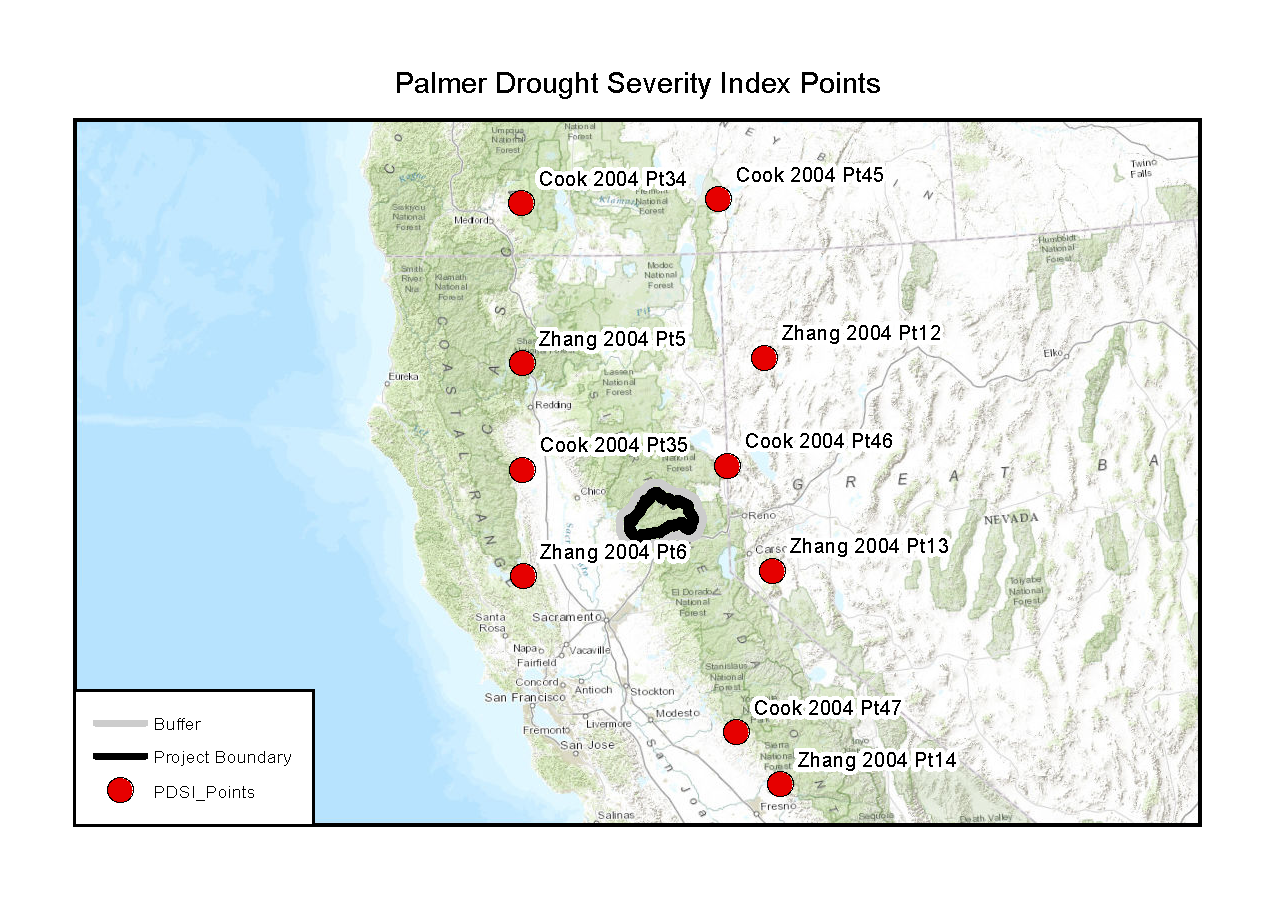
\includegraphics[width=\textwidth]{PDSIPointMap}
\end{figure}

\subsubsection{Calculations}
\begin{enumerate}
\item I combined all of the datasets into one Excel spreadsheet. 
\item Taking only the reconstructed data, I calculated the inverse distance weighted average of the PDSI values for each data point. 
\begin{enumerate}
\item Calculate the center point of the core area in ArcGIS.
\item Calculate the distance from each PDSI point to that center point. 
\item Rank the distances and standardize them by the closest point, such that the closest point is equal to 1 and the remaining points between 0 and 1. 
\item These effectively became the weight, and I calculated an overall average taking into account all of the weights by multiplying the PDSI value for a given year for each data point by this weighted value representing distance, summing them, and then dividing by the number of data points used. The number of data points used was not always the same because the Zhang data did not go as far back in time as the Cook data. 
\end{enumerate}
\item Convert yearly PDSI from 1550-1850 (historical period) into a 10-year average (PDSI per time step)
\item Recenter mean around 1 by rescaling 10-year PDSI values by 3-standard deviations: $y = \frac{x - \bar{x}}{2s + 1}$
\item Invert rescaled values so that positive values represent drought: $2\bar{x} - y$
\end{enumerate}

Finally, I created a comma-delimited text file containing only the time step values and the final PDSI values for import into RMLands.

\begin{figure}[h]
\centering
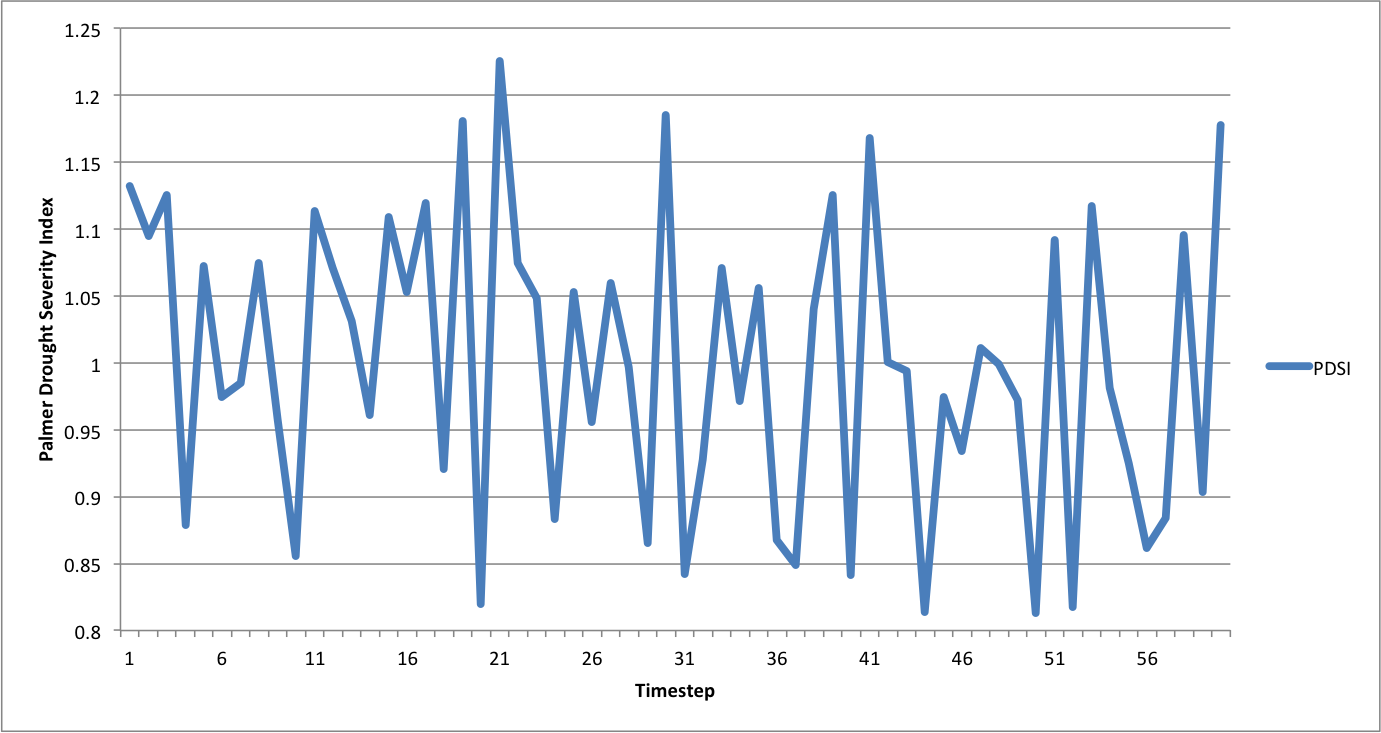
\includegraphics[width=0.8\textwidth]{PDSIpic}
\end{figure}

\subsection{Weather Stations}
I first looked into finding RAWS stations near the project area. Becky recommended using MesoWest, a service from the University of Utah that provides access to archived weather observations.

I consulted with a fuels specialist on the Tahoe as well as Becky in order to determine the dates of the fire season and hours for the daily burning period. On June 20th we resolved that fire season lasts from May 15 to October 15, and the burning period is 6-8 hours. Becky and I resolved to use 1000-1800 as the burning period.

Using MesoNet and Weather Underground, I identified several potential stations to use for weather data.
\begin{enumerate}
\item Rice Canyon (TT179): data going back to November 2012 
\item Saddleback: data going back to June 2001 (this is the station that gives the weather for Downieville, in the center of the project area)
\item Downieville [Wunderground] (KCADOWN12): data going back to 2009.
\item White Cloud: data going back to February 1993
\item Emigrant Gap: data going back to April 1997
\item Blue Canyon (KBLU): data going back to 1948
\end{enumerate}

From MesoWest, I downloaded data on the following variables:
\begin{itemize}
\item SKNT - wind direction in degrees
\item GUST - highest wind gust speed
\item DRCT - wind direction in categorial values (e.g. NW, SSE)
\item PEAK - highest sustained wind speed
\end{itemize}

\begin{figure}[h!]
\centering
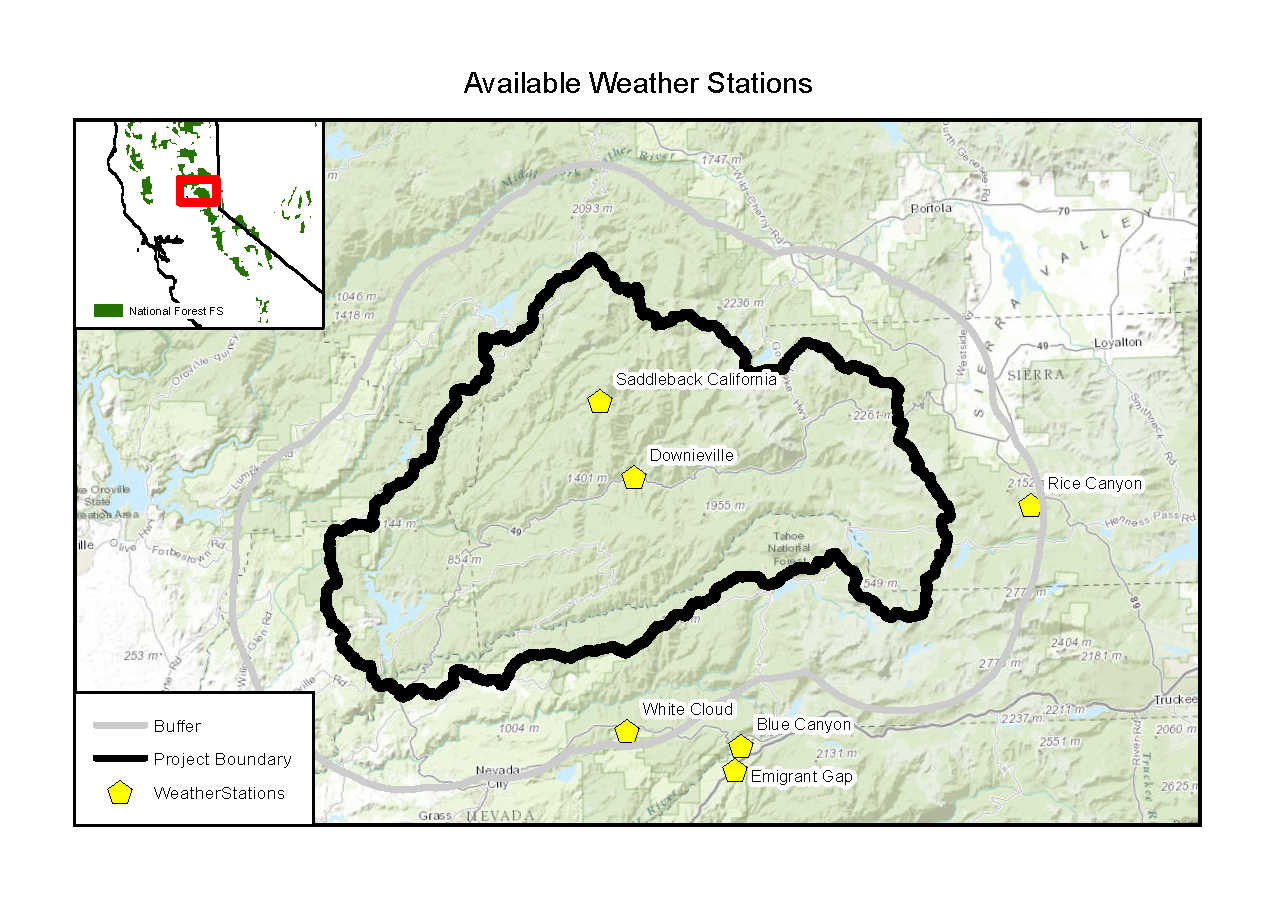
\includegraphics[width=\textwidth]{WeatherStationMap}
\end{figure}

Becky confirmed that all were close enough to the project area to be relevant.

The data for weather stations on Mesonet was obtained via a form for downloads on the mesonet website. I used a Python script to obtain the data stored on the Weather Underground site.
\begin{lstlisting}
import urllib2
#Create/open a file called wunder.txt (which will be a comma-delimited file), 
#in write mode
def weather(year):
#   works for 1948
    fname = '../Climate/WeatherStationData/wunder-data-%d.txt' % year
    f = open(fname, 'w')
    #Iterate through month, and day
    for m in range(5, 11):
        for d in range(1, 32):
            #Open wunderground.com url
            url = "http://www.wunderground.com/history/airport/KBLU/"+str(year)+"/" +str(m)+"/"+str(d)+"/DailyHistory.html?format=1"
            page = urllib2.urlopen(url)
            dailyData = page.read()
            f.write(dailyData)
    f.close()                            

#for year in range(1948, 1950):
#    weather(year)

def weather2(year):
#   works for 1949+
#   Create/open a file called wunder.txt (which will be a comma-delimited file), 
#   in write mode
    fname = '../Climate/WeatherStationData/wunder-data-%d.txt' % year
    f = open(fname, 'w')
    #Iterate through month, and day
    for m in range(5, 11):
        for d in range(1, 32):
            #Open wunderground.com url
            url = ''http://www.wunderground.com/history/airport/KBLU/'' + str(year) + ''/'' + str(m) + ''/'' + str(d) + ''/DailyHistory.html?req_city=NA&req_state=NA&req_statename=NA&format=1''
            page = urllib2.urlopen(url)
            dailyData = page.read()
            f.write(dailyData)
    f.close() 
\end{lstlisting}

I am primarily interested in the wind direction value, so even though there were many other data in each file, I created a new file storing only the wind direction data for the hours and dates in which I was interested.
\begin{lstlisting}
import glob
def wunderclean():
    ''' This function takes the output from the above functions and cleans it up so that it will only have the weather data from the hours that I will want it from. Range of times desired is 10:00 AM through 6:59 PM. The name of the first column (related to time of day) is inconsistent throughout the files. We have seen TimePDT, TimePST, and Time. We have decided not to convert TimePDT and PST to the same time. 'Time' seems to only appear once on a day in which the station malfunctioned and no data was recorded (June 6 1979). Another error arose from June 1998 in which the string printed ''No daily or hourly history data available,'' which we have corrected by adding 'No daily' to the list of cues to skip the line for data collection.
    '''
    outname = '../Climate/WeatherStationData/wunderclean.txt'
    #outname = '../Climate/WeatherStationData/'+ raw_input('new file name')
    out = open(outname, 'w')
    for fname in glob.glob('../Climate/WeatherStationData/wunder-data-*.txt'):
        print 'opening %s' %fname.split('/')[-1]
        f = open(fname, 'r')
        flines = f.readlines()
        for line in flines:
            if line.startswith('Time') or len(line) < 2 or line.startswith('No daily'):
                #print 'header or blank'
                continue
            elif not indaterange(line):
                #print 'out of range'
                continue
            hour = int(line.split(':')[0])
            if 10 <= hour < 12 and 'AM' in line:
                out.write(line)
            elif 12 == hour and 'PM' in line:
                # Special case Noon
                out.write(line)
            elif 1 <= hour <= 6 and 'PM' in line:
                out.write(line)
        f.close()
    out.close() 

def indaterange(line):
    """ Checks whether the line is from a date during the fire season. Currently only checks that the date is in May before May 15th (May 15th is OK)
    """
    baddates = [ '05-%02i' % i for i in range(15) ]
    for date in baddates:
        if date in line:
            return False
    return True

import glob
def mesonetclean(newfile, filepath):
    ''' This function takes the output from the above functions and cleans it up so that it will only have the weather data from the hours that I will want it from. Range of times desired is 10:00 AM through 6:59 PM
    '''
    outname = '../Climate/WeatherStationData/' + newfile
    #outname = '../Climate/WeatherStationData/'+ raw_input('new file name')
    out = open(outname, 'w')
    for fname in glob.glob('../Climate/WeatherStationData/'+ filepath):
        print 'opening %s' %fname.split('/')[-1]
        f = open(fname, 'r')
        flines = f.readlines()
        for line in flines:
            if line[0].isdigit():
                hour = int(line.split(',')[3])
                if 10 <= hour <= 18:
                    out.write(line)
                else:
                    continue
            else:
                continue
        f.close()
    out.close() 
\end{lstlisting}

Finally, I wrote a Python script to extract the wind direction in degrees from the downloaded weather data, bin it into categories, and generate the relative proportion on a 0-1 scale of wind direction.

\begin{lstlisting}
Bins for wind direction
(1) N [337.5-22.5 degrees]
(2) NE [22.5-67.5 degrees]
(3) E [67.5-112.5 degrees]
(4) SE [112.5-157.5 degrees]
(5) S [157.5-202.5 degrees]
(6) SW [202.5-247.5 degrees]
(7) W [247.5-292.5 degrees]
(8) NW [292.5-337.5 degrees]
(9) Flat [i.e., slope = 0]
(NODATA) cells outside of project boundary

===============================================================
import numpy as np

#variables

windN = 0
windNE = 0
windE = 0
windSE = 0
windS = 0
windSW = 0
windW = 0
windNW = 0
windFLAT = 0
windcounts = { d : 0 for d in ['N','NE','E','SE','S','SW','W','NW'] }

kbludata = np.genfromtxt("WeatherStationData/wunderclean.txt", dtype=int, delimiter = ',', skip_header = 1, usecols = 12) 

#note for mesowest variables DRCT is the wind direction
slecdata = np.genfromtxt("WeatherStationData/SLEC1.txt", dtype=int, delimiter = ',', usecols = 8, missing_values='', filling_values='0') 
ciscdata = np.genfromtxt("WeatherStationData/CISC1.txt", dtype=int, delimiter = ',', usecols = 8, missing_values='', filling_values='0') 
#slecdata_save = np.savetxt("WeatherStationData/SLEC1_WindSpd.txt", slecdata, delimiter=',')

for item in kbludata:
    winddir = item
    if (winddir > 337.5) or (winddir <= 22.5) & (winddir > 0):
        windN += 1
    elif (winddir > 22.5) and (winddir <= 67.5):
        windNE += 1
    elif (winddir > 67.5) & (winddir <= 112.5):
        windE += 1
    elif (winddir > 112.5) & (winddir <= 157.5):
        windSE += 1
    elif (winddir > 157.5) & (winddir <= 202.5):
        windS += 1
    elif (winddir > 202.5) & (winddir <= 247.5):
        windSW += 1
    elif (winddir > 247.5) & (winddir <= 292.5):
        windW += 1
    elif (winddir > 292.5) & (winddir <= 337.5):
        windNW += 1
    elif (winddir == 0):
        windFLAT += 1
    else:
        print "Wind direction not an allowed value."    
print "Totals after KBLU:"
print "windN =", windN, "windNE =", windNE, "windE =", windE, "windSE =", windSE, "windS =", windS, "windSW =", windSW, "windW =", windW, "windNW =", windNW, "windFLAT =", windFLAT

for item in slecdata:
    winddir = item
    if (winddir > 337.5) | (winddir <= 22.5) & (winddir > 0):
        windN += 1
    elif (winddir > 22.5) & (winddir <= 67.5):
        windNE += 1
    elif (winddir > 67.5) & (winddir <= 112.5):
        windE += 1
    elif (winddir > 112.5) & (winddir <= 157.5):
        windSE += 1
    elif (winddir > 157.5) & (winddir <= 202.5):
        windS += 1
    elif (winddir > 202.5) & (winddir <= 247.5):
        windSW += 1
    elif (winddir > 247.5) & (winddir <= 292.5):
        windW += 1
    elif (winddir > 292.5) & (winddir <= 337.5):
        windNW += 1
    elif (winddir == 0):
        windFLAT += 1
    else:
        print "Wind direction not an allowed value."    
print "Totals after KBLU, SLEC:"
print "windN =", windN, "windNE =", windNE, "windE =", windE, "windSE =", windSE, "windS =", windS, "windSW =", windSW, "windW =", windW, "windNW =", windNW, "windFLAT =", windFLAT

for item in ciscdata:
    winddir = item
    if (winddir > 337.5) | (winddir <= 22.5) & (winddir > 0):
        windN += 1
    elif (winddir > 22.5) & (winddir <= 67.5):
        windNE += 1
    elif (winddir > 67.5) & (winddir <= 112.5):
        windE += 1
    elif (winddir > 112.5) & (winddir <= 157.5):
        windSE += 1
    elif (winddir > 157.5) & (winddir <= 202.5):
        windS += 1
    elif (winddir > 202.5) & (winddir <= 247.5):
        windSW += 1
    elif (winddir > 247.5) & (winddir <= 292.5):
        windW += 1
    elif (winddir > 292.5) & (winddir <= 337.5):
        windNW += 1
    elif (winddir == 0):
        windFLAT += 1
    else:
        print "Wind direction not an allowed value."    
print "Totals after KBLU, SLEC, CISC:"
print "windN =", windN, "windNE =", windNE, "windE =", windE, "windSE =", windSE, "windS =", windS, "windSW =", windSW, "windW =", windW, "windNW =", windNW, "windFLAT =", windFLAT

==============================================================

RESULTS At 1612 on 8/23/2013:
Totals after KBLU, SLEC, CISC:
windN = 3612 windNE = 4616 windE = 5340 windSE = 6039 windS = 33015 windSW = 26450 windW = 25230 windNW = 6420 windFLAT = 10262

============================================

windarray = [3612., 4616., 5340., 6039., 33015., 26450., 25230., 6420.]
windsum = sum(windarray)
windpercent = divide(windarray, windsum)
[ 0.03262224  0.04169     0.0482289   0.05454201  0.29817922  0.23888658  0.22786799  0.05798306]

 N 0.03262224
 NE 0.04169
 E 0.0482289
 SE 0.05454201
 S 0.29817922
 SW 0.23888658
 W 0.22786799
 NW 0.05798306
\end{lstlisting}

\section{Fire Size}
To calculate the proportion of fires within a set of bins ordered by magnitude (1, 10, 100, 1,000, 10,000, and 100,000 hectares), I used real data. Data on fire sizes in California goes back to approximately 1904 in the state. However, I did not want to use fire sizes from the entire state, since it is so large and encompasses so many diverse ecosystems. The Existing Vegetation layers were developed for the whole state as well, and published in subsections by ecotype. One of those ecotypes is the North Sierra, also known as Zone 3. The CalVeg alliances were tied to this zone as well. I then used the Pacific Crest Trail as a conservative eastern boundary (the trail is often to the east of the actual crest in the study landscape), redrawing the polygon. I then clipped the fire occurrence data to the new polygon, and sorted the fires using a python script.

\begin{lstlisting}
point = np.genfromtxt("point_table_0923_1743.txt", delimiter=',', skip_header=1, usecols=30, comments=None)
poly = np.genfromtxt("poly_table_0923_1743.txt", delimiter=',', skip_header=1, usecols=15, comments=None)
both = np.append(point, poly)
both_ha = both * 0.404686
bins = [0, 1, 10, 100, 1000, 10000, 100000]
\end{lstlisting}



The output of the histogram function gives the number of fires falling within each size range.
\begin{lstlisting}
In: np.histogram(both_ha, bins=bins)
Out: 
(array([8107,  609,  460,  398,  102,   13]),
 array([     0,      1,     10,    100,   1000,  10000, 100000]))
\end{lstlisting}

Finally, I computed the proportion of fires in each bin.
\begin{lstlisting}
binnedfire, bins = np.histogram(both_ha, bins=bins)
In: rml_firevals = binnedfire / np.sum(binnedfire, dtype=np.float)
Out: array([ 0.83672206,  0.06285478,  0.04747652,  0.04107751,  0.0105274 , 0.00134173])
In: rml_firevals_pct = rml_firevals * 100
Out: array([ 83.67220559,   6.28547838,   4.74765198,   4.10775106, 1.05274022,   0.13417277])
\end{lstlisting}        

\section{Susceptibility}
\subsection{Hazard Function}
One input in the model is to apply the hazard function of the Weibull model to the susceptibility to fire for a given cover type. The inputs are scale (equivalent to mean FRI), shape (which has no deterministic basis, and is typically 3), and the reset point for the function (age since any disturbance, age since high mortality, age since low mortality, age since condition class change, etc). There is an accompanying graphic within RMLands that shows what this curve looks like for a given cover type parameter selection. While we were parameterizing the adapted model the first time, Kevin realized that prior uses of the model had technically misused the hazard function, which is an unbounded on the right function. In previous versions, RMLands simply truncated the hazard function when the output value reached 1 (because it is treated as a probability in the model). It did not cause problems in prior runs, but appeared to in our initial Sieran runs. Consequently, we will modify RMLands such that in future simulations the cumulative form of the Weibull model will be used instead. It contains the same parameters as the hazard.

For at least the initial parameterization of the model, we used the expert and literature-generated FRI values. When choosing ``age since \_\_\_\_\_\_,'' we selected ``Age since any disturbance'' for fuel-driven cover types, and ``Age since high mortality disturbance'' for climate and weather-drive cover types.

\subsection{Spread Weights}
Where the model asks for inputs for Min and Max, this refers to fire size. Recall that each fire is probablistically assigned a maximum size at the time of initiation. Reviewing the fire size distribution for most areas reveals that most fires fall on the ``min'' side.

\section{Spread}
Use joint cell: if multiple adjacent burning cells, a given unburnt cell is more likely to burn. it get evaluated multiple times and the probabilities are summed.
Cell evaluation: cells are reevaluated each step
Majority filter - 3x3 window to smooth fire edges and fill in holes
Local spread window: to deal with pixelated landscapes - mostly for bugs


         